\documentclass[a4paper]{article}

%% Language and font encodings
\usepackage[english]{babel}
\usepackage[utf8x]{inputenc}
\usepackage[T1]{fontenc}

%% Sets page size and margins
\usepackage[a4paper,top=3cm,bottom=2cm,left=3cm,right=3cm,marginparwidth=1.75cm]{geometry}

%% Useful packages
\usepackage{amsmath}
\usepackage{graphicx}
\usepackage[colorinlistoftodos]{todonotes}
\usepackage[colorlinks=true, allcolors=blue]{hyperref}

\title{Actividad 8}
\author{Isaac Neri Gómez Sarmiento}
\date{15 de Abril 2018}

\begin{document}
\maketitle

\section{Introducción: Antecedentes}

En esta actividad continuamos modelando sistemas físicos con ecuaciones diferenciales no lineales. Tal es el caso del oscilador de Van der Pol.

Tal y como el nombre lo indica, este fue propuesto por el físico holandés Balthasar van der Pol y es un oscilador con amortiguamiento no lineal.

Van der Pol estaba interesado en buscar una forma de regular las arritmias o  latidos irregulares del corazón, he de ahí los inicios que condujeron a los marcapasos. 

Tiene otras aplicaciones en varios campos de la ciencia, como en la geología al ser usado en el desarrollo de un modelo de interacción entre 2 placas en una falla geológica.




\section{Modelo de Van der Pol}

Este modelo es un oscilador no conservativo con un amortiguamiento no lineal. Esta representado por la siguiente ecuación diferencial de segundo orden y evoluciona conforme pasa el tiempo.


\begin{figure}[ht!]
\centering
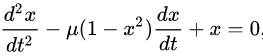
\includegraphics[width=0.4\textwidth]{Eq_dif1.PNG}
\end{figure}


Pero se puede reescribir como un sistema de dos ecuaciones de primer orden:


\begin{figure}[ht!]
\centering
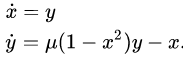
\includegraphics[width=0.30\textwidth]{Eq_dif2.PNG}
\end{figure}

\noindent
Lamentablemente el modelo no tiene una solución a analítica exacta. 

El oscilador de van der Pol puede ser un oscilador armónico simple solo en el caso en el que la constante de amortiguamiento $\mu$ sea igual a cero.

En el caso que $\mu>0$, el sistema entrará en un ciclo límite. En el orígen el sistema parece ser inestable y conforme se aleja, el sistema es amortiguado.

Se puede hablar de un oscilador de Van der Pol forzado, al cual  se le puede añadir una función del tipo Asin($\omega$t) y quedaría de la siguiente forma:


\begin{figure}[ht!]
\centering
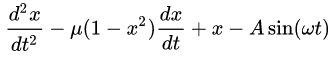
\includegraphics[width=0.45\textwidth]{Eq_dif3.PNG}
\end{figure}

En los circuitos eléctricos, para que pueden ser descritos por la ecuación de Van der Pol, se necesitan elementos activos del circuito con la propiedad cúbica no lineal:

\begin{figure}[ht!]
\centering
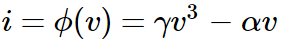
\includegraphics[width=0.3\textwidth]{Eq_dif5.PNG}
\end{figure}





\newpage

\section {Exploración de las soluciones del modelo en el Espacio Fase}

En esta sección probaremos soluciones con 3 valores distintos de mu:


\begin{figure}[ht!]
\centering
\centering
\includegraphics[width = 0.5\textwidth]{Figxploremu__001.png}
\caption{Phaseplot con $\mu=0.001$}
\end{figure}

\begin{figure}[ht!]
\centering
\centering
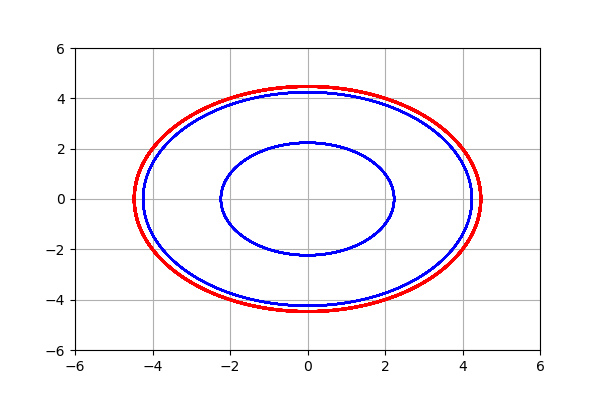
\includegraphics[width = 0.5\textwidth]{Figxploremu_0.png}
\caption{Phaseplot con $\mu=0$}
\end{figure}

\begin{figure}[ht!]
\centering
\centering
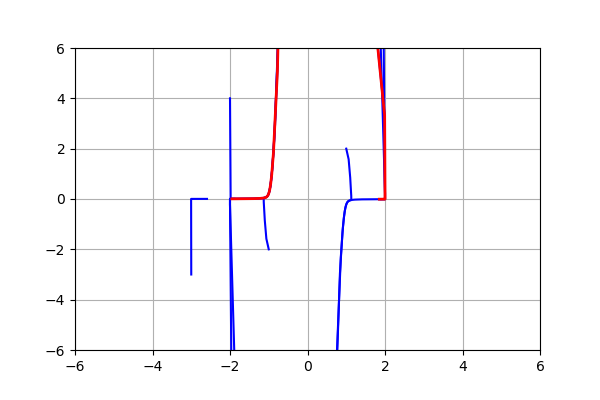
\includegraphics[width = 0.5\textwidth]{Figxploremu_100.png}
\caption{Phaseplot con $\mu=100$}
\end{figure}


Las condiciones iniciales se mantuvieron igual que en el ejemplo de Wikipedia, con la diferencia de los valores distintos de $\mu$. 
Podemos observar que el phaseplot con valor de mu cercano a cero se parece al que si tiene valor de mu igual a cero.

Recordemos que cuando el parámetro de amortiguamiento $\mu=0$, la ecuación que describe el oscilador de Van der Pol adquiere la forma de un oscilador armónico simple y existe conservación de la energía.
\newpage

\begin{figure}[ht!]
\centering
\centering
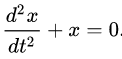
\includegraphics[width = 0.2\textwidth]{Eq_dif4.PNG}


Para la tercera figura, utilizamos un valor grande de mu, especificamente $\mu=100$.

El ciclo límite en rojo no parece cerrarse.

\end{figure}

\section{Resultados y discusión}
Para la resolución de la ecuación diferencial, se utilizó el sistema de dos ecuaciones de primer orden. El código es muy similar al utilizado en otras prácticas anteriores:

\begin{verbatim}
from scipy.integrate import odeint
import numpy as np

def vectorfield(w, t, p):
    """
    Arguments:
        w :  vector of the state variables:
                  w = [x,y]
        t :  time
        p :  vector of the parameters:
                  p = [mu]
    """
    x, y = w

    # Create f = (x',y'):
    f = [y,
         (p*(1.0 - x**2.0) * y) - x]
    return f
\end{verbatim}


Para generar las soluciones, en un caso específico donde los parámetros eran:

\begin{center}
$\mu=0.1$

x=2

y=-3
\end{center}

\begin{verbatim}
#Lista de datos generados por el ODE solver para el parametro
# ****************** mu=0.1 *******************

mu = 0.1
# Initial conditions
# x is the initial displacement and y is the initial velocity
x = 2.0
y = -3.0

stoptime = 100
numpoints = 3000

# Create the time samples for the output of the ODE solver.
# I use a large number of points, only because I want to make
# a plot of the solution that looks nice.
t = [stoptime * float(i) / (numpoints - 1) for i in range(numpoints)]

# Pack up the parameters and initial conditions:
w0 = [x, y]

# Call the ODE solver.
wsol = odeint(vectorfield, w0, t, args=(mu,))

with open('vanderpol_0', 'w') as f:
    # Print & save the solution.
    for t1, w1 in zip(t, wsol):
        print (t1, w1[0], w1[1], file=f)
\end{verbatim}

Se obtuvieron cuatro gráficas, simulando las de Wikipedia, las cuales son las siguientes:

\begin{figure}[ht!]
\centering
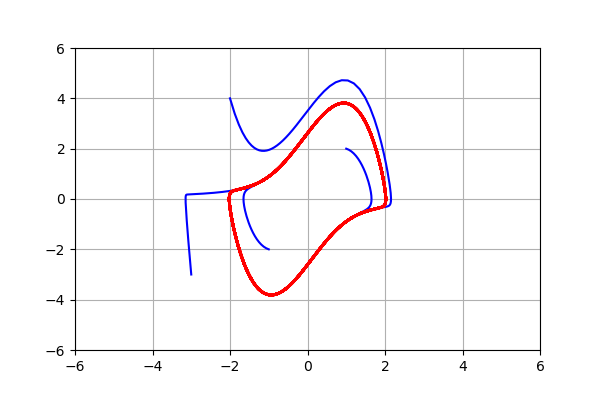
\includegraphics[width=0.45\textwidth]{Figura1.png}
\end{figure}

Esta gráfica es un diagrama de fase del oscilador de Van der Pol no forzado, mostrando el ciclo limite en rojo, es decir la trayectoria cerrada a la cual tienden las demás sea dentro de ella o por fuera de ella cuando se considera un tiempo considerablemente grande.



\begin{figure}[ht!]
\centering
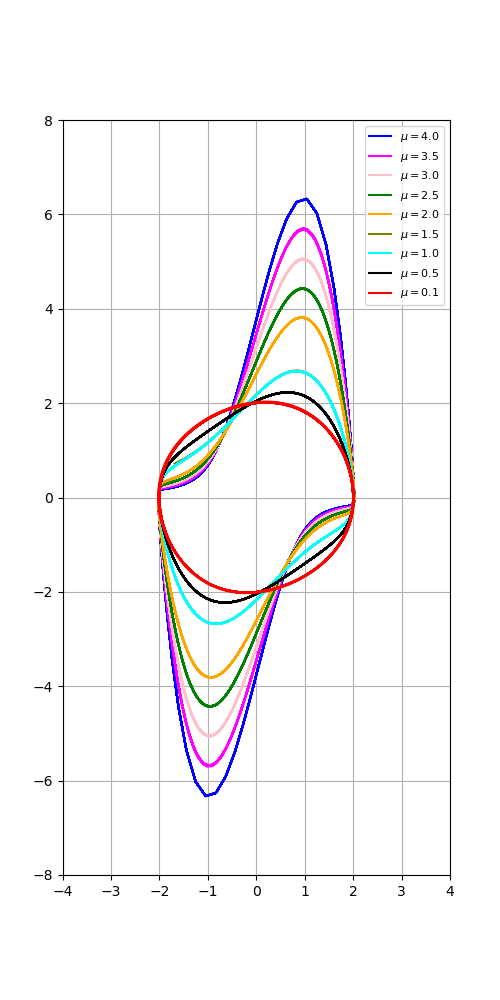
\includegraphics[width=0.4\textwidth]{Figura2.png}
\end{figure}

En la gráfica de arriba podemos observar como el cíclo límite varía cuando se escogen diferentes valores de $\mu$. Para el valor de $\mu=0.1$ podemos ver que el cíclo límite tiene forma de circunferencia. Conforme el valor de $\mu$ va aumentando, el ciclo límite va adquiriendo unos picos en los extremos.
Este es un ejemplo de oscilador de relajación, el cual  se representa en forma gráfica como una curva no sinusoidal repetitiva tal como una onda triagular o cuadrada.

\newpage
En la siguiente imágen podemos ver un ejemplo claro de la gráfica de un oscilador de relajación cuyo parámetro de amortiguamiento es $\mu=5$.


\begin{figure}[ht!]
\centering
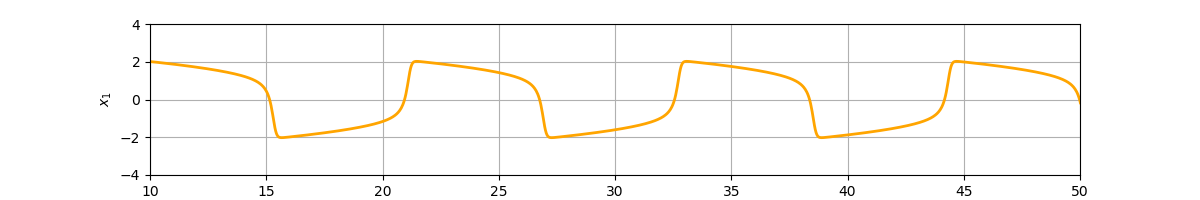
\includegraphics[width=1\textwidth]{Figura3.png}
\end{figure}

En la gráfica de abajo se observa un oscilador de Van der Pol con forzamiento.
El forzamiento usado es del tipo senoidal y se utilizaron los siguientes parámetros: \\

\begin{center}
$\mu=8.53$
$A=1.2$
$ \omega=2\pi/10$
\end{center}




\begin{figure}[ht!]
\centering
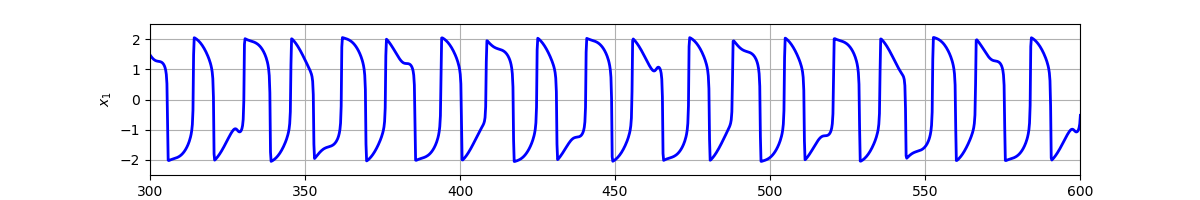
\includegraphics[width=1\textwidth]{Figura4.png}
\end{figure}



\section{Conclusiones}
Los diagramas de fase son importantes en la representación de sistemas dinámicos con ecuaciones diferenciales. Estos nos permiten identificar por ejemplo ciclos límites, los cuales son trayectorias cerradas en donde al menos una otra trayectoria gira alrededor de ella cuando el tiempo se aproxima a infinito.

El oscilador de Van der Pol tiene un comportamiento caótico debido a la sensibilidad que tiene a las condiciones iniciales. Puede considerarse como un oscilador armónico simple cuando $\mu=0$. Al probar con valores muy grandes de la constante de amortiguamiento, parece ser que no se cierra la trayectoría. 
Este oscilador tiene oscilación de relajación y se puede apreciar en una gráfica de desplazamiento contra tiempo ya que las oscilaciones no tienen forma de onda sinusoidal.


\section{Bibliografía}

\textit{Van der Pol oscillator. } Recuperado el 14 de abril 2018 de:

\url{https://en.wikipedia.org/wiki/Van_der_Pol_oscillator}

\url{http://www.scholarpedia.org/article/Van_der_Pol_oscillator}



\textit{Lokta Volterra}. Recuperado el 11 de abril 2018 de:

\url{http://scipy-cookbook.readthedocs.io/items/LoktaVolterraTutorial.html}




\section{Apéndice}

\textbf{1° Este ejercicio pareciera similar al desarrollado en las actividades 6 y 7. ¿Qué aprendiste nuevo?}

Aprendí un poco más sobre los ciclos límites y los diagramas de fase utilizando el modelo de oscilador de Van der Pol. Además que a partir de este, usando ciertos parámetros, se puede obtener un oscilador armónico simple.\\

\textbf{2° ¿Qué fue lo que más te llamó la atención del oscilador de Van der Pol?}

Que tenga bastantes aplicaciones, ya sea en medicina o sismología. En cuanto a las gráficas y ecuación, me llamó la atención que pudiéramos reducir la ecuación diferencial de segundo orden a un sistema de dos ecuaciones de primer orden. También que variando un poco las condiciones iniciales, cambia notablemente la representación gráfica.\\

\textbf{3° Has escuchado ya hablar de caos. ¿Por qué sería importante estudiar este oscilador?}

La palabra como se usa comunmente para denotar “desastre” si, en el contexto de física o matemáticas también, y considero que se refiere a que un modelo que es caótico, es que no se comporta de manera simple, sino que es difícil de encontrar algún patrón que lo pueda describir, además de ser muy susceptible a las condiciones iniciales.\\

\textbf{4° ¿Qué mejorarías en esta actividad?}

Me gustaría leer algún paper de cómo se aplica paso a paso este modelo en un ejemplo sencillo.\\

\textbf{5° ¿Algún comentario adicional antes de dejar de trabajar en Jupyter con Python?}

Me hubiera gustado aprender algoritmos para resolver ecuaciones diferenciales en lugar de utilizar la librería scipy.integrate.ode.\\

\textbf{6° Cerramos la parte de trabajo con Python ¿Que te ha parecido?}

Me parecieron interesantes las actividades que realizamos. Considero que hubiera aprovechado un poco más el curso aprendiendo de manera general la sintaxis de Python, cómo hacer funciones, subrutinas, etc, para así tener más libertad de programación y no solo utilizar los ejemplos como una “caja negra”.








\end{document}